% Fact sheet for MATH 300, for Fall 2014.
\documentclass{article}[12pt]

% useful packages
\usepackage{fullpage}
\usepackage{amsmath,amssymb,amsthm,amsfonts}
\usepackage{graphicx}
\usepackage{enumerate}
\usepackage{algorithm,algorithmicx}
\usepackage{xcolor}
\usepackage{bbm}
\usepackage{url}
\usepackage{caption,subcaption}
\usepackage{booktabs}

% theorem type environments
\newtheorem{thm}{Theorem}
\newtheorem{prop}{Proposition}
\newtheorem{lemma}{Lemma}
\newtheorem{cor}{Corollary}
\newtheorem{defn}{Definition}
\newtheorem{assump}{Assumption}
\newtheorem{example}{Example}
\newtheorem{conjecture}{Conjecture}

% frequently used symbols
\newcommand{\bE}{\mathbb{E}}
\newcommand{\bP}{\mathbb{P}}
\newcommand{\bQ}{\mathbb{Q}}
\newcommand{\bR}{\mathbb{R}}
\newcommand{\bS}{\mathbb{S}}
\newcommand{\bN}{\mathbb{N}}
\newcommand{\bZ}{\mathbb{Z}}
\newcommand{\sC}{{\mathcal C}} 
\newcommand{\sD}{{\mathcal D}} 
\newcommand{\sE}{{\mathcal E}} 
\newcommand{\sF}{{\mathcal F}} 
\newcommand{\sL}{{\mathcal L}} 
\newcommand{\sH}{{\mathcal H}} 
\newcommand{\sN}{{\mathcal N}} 
\newcommand{\sO}{{\mathcal O}} 
\newcommand{\sP}{{\mathcal P}} 
\newcommand{\sR}{{\mathcal R}} 
\newcommand{\sS}{{\mathcal S}}
\newcommand{\sU}{{\mathcal U}} 
\newcommand{\sX}{{\mathcal X}} 
\newcommand{\sY}{{\mathcal Y}} 
\newcommand{\sZ}{{\mathcal Z}}

% operators
\newcommand{\sign}{\mathop{\mathrm{sign}}}
\newcommand{\supp}{\mathop{\mathrm{supp}}} % support
\newcommand{\argmin}{\operatornamewithlimits{arg\ min}}
\newcommand{\argmax}{\operatornamewithlimits{arg\ max}}
\newcommand{\dist}{\operatorname{dist}}
\newcommand{\tr}{\text{tr}}
\newcommand{\vecop}{\text{vec}}
\newcommand{\st}{\operatorname{s.t.}}
\newcommand{\cut}{\setminus}
\newcommand{\ra}{\rightarrow}
\newcommand{\ind}[1]{\mathbbm{1}\left\{#1\right\}} 
\newcommand{\given}{\ | \ }

% grouping operators
\newcommand{\brac}[1]{\left[#1\right]}
\newcommand{\set}[1]{\left\{#1\right\}}
\newcommand{\abs}[1]{\left\lvert #1 \right\rvert}
\newcommand{\paren}[1]{\left(#1\right)}
\newcommand{\norm}[1]{\left\|#1\right\|}
\newcommand{\ip}[2]{\left\langle #1,#2 \right\rangle}

% code commands
\newcommand{\matlab}{\textsc{Matlab }}
\newcommand{\algname}[1]{\textnormal{\textsc{#1}}}

\graphicspath{{./img/}}

\makeatletter
\renewcommand*\env@matrix[1][*\c@MaxMatrixCols c]{%
	  \hskip -\arraycolsep
	    \let\@ifnextchar\new@ifnextchar
	      \array{#1}}
	      \makeatother

% header command
\newcommand{\homework}[4]{
    \pagestyle{myheadings}
    \thispagestyle{plain}
    \newpage
    \setcounter{page}{1}
    \setlength{\headsep}{10mm}
    \noindent
    \begin{center}
    \framebox{
        \vbox{\vspace{2mm}
            \hbox to 6.28in { {\bf STAT 672: Statistical Learning II
            \hfill Winter 2020} }
        \vspace{4mm}
        \hbox to 6.28in { {\Large \hfill Homework #1 \hfill} }
        \vspace{2mm}
        \hbox to 6.28in { \Large \hfill Due: #2 \hfill }
        \vspace{2mm}
        \hbox to 6.28in { {\it Student Name: #3} \hfill {\it Professor Name: #4}}
        \vspace{2mm}}
   }
   \end{center}
   \markboth{Homework #1}{Homework #1}
   \vspace*{4mm}
}

\begin{document}
\homework{4}{February 19th, 2020}{Ethan Lew}{Bruno Jedynak}
\section{Multivariate Normal random Vectors (MVN)}

Let $X \sim MVN(\mu,\Sigma)$. Let $\lambda_1 \geq \ldots \lambda_m > 0 = \lambda_{m+1} = \ldots = \lambda_n$ be the e-values of $\Sigma$. Let $u_1,\ldots,u_m$ be the e-vectors associated with these e-values and let 
\begin{equation} \label{eq:mvny}
Y_i = (X-\mu)^T u_i, 1 \leq i \leq m
\end{equation}
then,  show the following: 
\begin{enumerate}
\item $Y_1,\ldots,Y_m$ are independent;

\textbf{Solution: }First, it is evident that $Y_i, i \le i \le m$ is normally distributed as the linear combination of gaussian random  variables is also a gaussian random variable,
	\begin{equation}
		Y_i = (X - \mu)^T u_i = \sum^{d}_{k=1} X_k \left[ u_i \right]_k - \mu^T u_i. 
	\end{equation}
	
	In the case of Multivariate Normal random variables, uncorrelatedness does imply independence. Hence, it is sufficient to show that the covariance between any two $Y_i, Y_j$ is zero, assuming $i \ne j$. Start by substituting Equation \ref{eq:mvny} into the covariance expression,
	\begin{equation}
		\begin{aligned}
			\operatorname{cov} \left( Y_i, Y_j \right) &= \operatorname{cov} \left[ \left( x - \mu \right)^T u_i, \left( X - \mu \right)^T u_j \right] \\
								   &= \operatorname{cov} \left( X^T u_i, X^T u_j \right) 
								   - \operatorname{cov} \left( X^T u_i, \mu^T u_j \right) - \operatorname{cov} \left( \mu^T u_i, X^T u_j \right) + \operatorname{cov} \left( \mu^T u_i, \mu^T u_j \right)\\
								   &= \operatorname{cov} \left( X^T u_i, X^T u_j \right).\\
		\end{aligned}
	\end{equation}
Use the summation notation for the inner product as well as the bilinear property of the covariance operator,
\begin{equation}
	\begin{aligned}
		\operatorname{cov} \left( Y_i, Y_j \right) &= \operatorname{cov} \left[ \sum^{d}_{k=1} X_k \left[ u_i \right]_k, \sum^{d}_{k=1} X_k \left[ u_j \right]_k   \right] \\
							   &= \sum^{d}_{k=1} \sum^{d}_{l=1} \left[ u_i \right]_k \left[ u_j \right]_k \operatorname{cov} \left[ X_k, X_l \right].\\  
							   &= u_i^T \Sigma u_j.
	\end{aligned}
\end{equation}
Let the eigendecomposition of $\Sigma = U \Lambda U^T$,
\begin{equation} \label{eq:sigdecomp}
	\begin{aligned}
		\operatorname{cov} \left( Y_i, Y_j \right)	&= u_i^T U \Lambda U^T u_j \\
								&= e_i^T \Lambda e_j \\
								&= \lambda_j e_i^T e_j. \\
	\end{aligned}
\end{equation}
Now, $i \ne j$,
\begin{equation}
	\operatorname{cov} \left( Y_i, Y_j \right) = 0,\\
\end{equation}
being sufficient to imply that $Y_i, Y_j$ are independent.

\item $Y_i \sim N(0,\lambda_i)$

	\textbf{Solution: }Determine the expected value of $Y_i$,
	\begin{equation}
		\begin{aligned}
			\mathbb E \left[ Y_i \right] &= \mathbb E \left[ \left( X- \mu \right)^T u_i \right] \\
						     &= \mathbb E \left[ X^T u_i \right] - \mathbb E \left[ \mu^T u_i \right] \\
						     &= \sum^{d}_{k=1} \left[ u_i \right]_k \mathbb E \left[ X_k \right] - \mu^T u_i \\
						     &= \mu^T u_i - \mu^T u_i \\
						     &= 0. \\
		\end{aligned}
	\end{equation}
Now, for the variance of $Y_i$. Using Equation \ref{eq:sigdecomp},
\begin{equation}
	\begin{aligned}
		\operatorname{Var} \left[ Y_i \right] &= \operatorname{cov} \left[ Y_i, Y_i \right] \\
						      &= \lambda_i e^T_i e_i \\
						      &= \lambda_i.
	\end{aligned}
\end{equation}
Hence, $Y_i \sim N(0, \lambda_i) $.
	
\item 
\begin{equation}
\label{eq:sample}
X = \mu + Y_1 u_1 + \ldots + Y_m u_m
\end{equation}
\textbf{Solution: } It is sufficient to show that the first and second statistical moments of the LHS and RHS are equal to one another; It is known that both sides are Gaussian. For the expected value,
\begin{equation}
	\begin{aligned}
		\mathbb E \left[ X \right] &= \mu \\
		\mathbb E \left[ \mu + Y_1 u_1 + ... + Y_m u_m \right] &= \mu + \mathbb E \left[ Y_1 u_1 \right] + ... + \mathbb E \left[ Y_m u_m \right]. 
								       &= 0.\\
	\end{aligned}
\end{equation}

Next, the covariance, remember that the cross terms are zero,
\begin{equation}
	\begin{aligned}
		\operatorname{cov} \left[ X + Y_1 u_1 + ... + Y_m u_m \right] &= \operatorname{cov} \left[ \mu, \mu \right] + \operatorname{cov} \left[ Y_1 u_1, Y_1, u_1 \right] + ... + \operatorname{cov} \left[ Y_m u_m, Y_m, u_m \right] \\
									      &= U \Sigma U^T \\
									      &= \Sigma \\
									      &= \operatorname{cov} \left[ X \right].
	\end{aligned}
\end{equation}
Having shown the expected value and covariance to be zero, it is sufficient to show that the distributions of the LHS and RHS of the problem statement are the same.



One can use this construction to sample from a collection of images. Sample 500 images of the digit ``7\rq\rq{} from the MNIST dataset. 
Compute the empirical mean $\mu$ and the empirical covariance $\Sigma$. Consider the random vector $X \in \mathbb{R}^{784}$, with $X \sim MVN (\mu,\Sigma)$. 
Show $\mu$ as well as the 16 e-vectors associated with the largest e-values.  Sample 16 images from this distribution using (\ref{eq:sample}). Note: you might need to re-scale the e-vectors before plotting as they are of unit norm.  Truly, it doesn\rq{}t work so well in the sense that the samples of ``7\rq\rq{} do not look like real samples drawn by hand. More work is needed to obtain realistic samples.

\textbf{Solution: }See Figures \ref{fig:mean}, \ref{fig:evec} and \ref{fig:samps}.
\begin{figure}
	\centering
	\includegraphics[width=0.4\linewidth]{./img/digit_7.eps}
	\caption{The Mean Image of 500 Samples of the Digit ``7''.}%
	\label{fig:mean}
\end{figure}
\begin{figure}
	\centering
	\includegraphics[width=0.6\linewidth]{./img/evectors_7.eps}
	\caption{The First 16 Eigenvectors for the Digit ``7''.}%
	\label{fig:evec}
\end{figure}
\begin{figure}
	\centering
	\includegraphics[width=0.6\linewidth]{./img/samples_7.eps}
	\caption{16 Samples for the Digit ``7''.}%
	\label{fig:samps}
\end{figure}

% \begin{figure}
%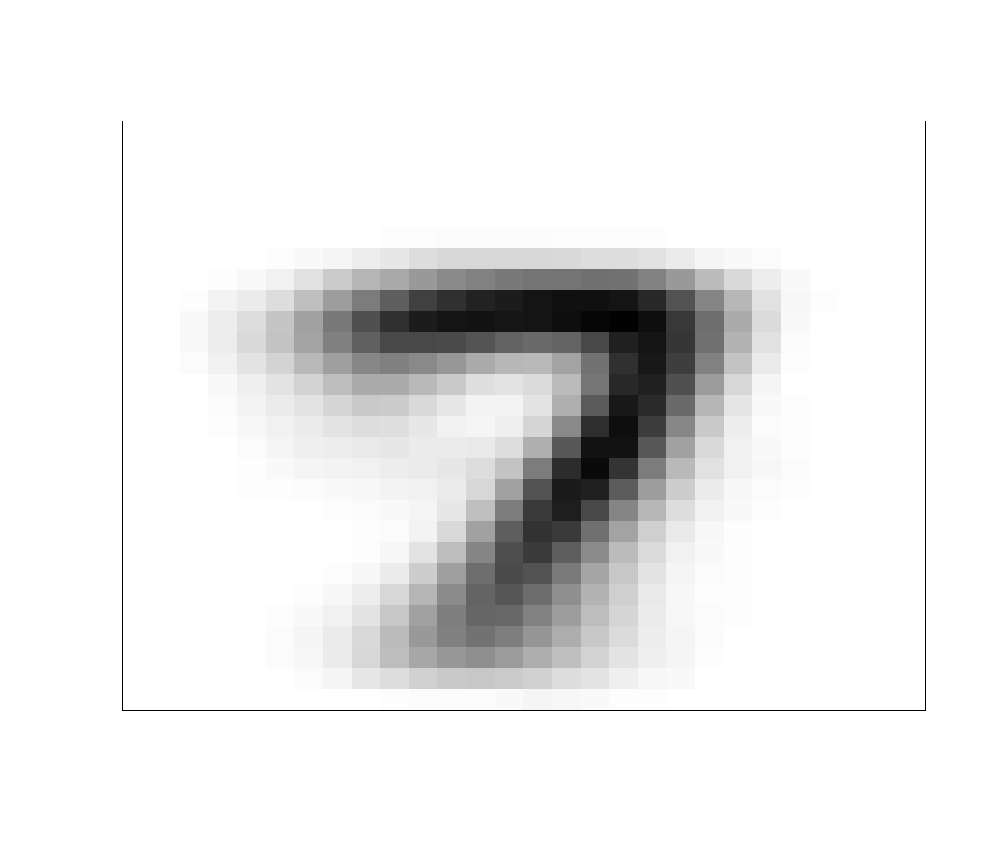
\includegraphics[width=0.5\textwidth]{mu.pdf}
%\caption{\label{fig:mu}the mean image of 500 images of the digit ``7\rq\rq{}}
%\end{figure}
%\begin{figure}
%
\includegraphics[width=0.8\textwidth]{e-vectors.pdf}
%\caption{\label{fig:e-vectors}The 16 first e-vectors for the digit ``7\rq\rq{}}
%\end{figure}
%\begin{figure}
%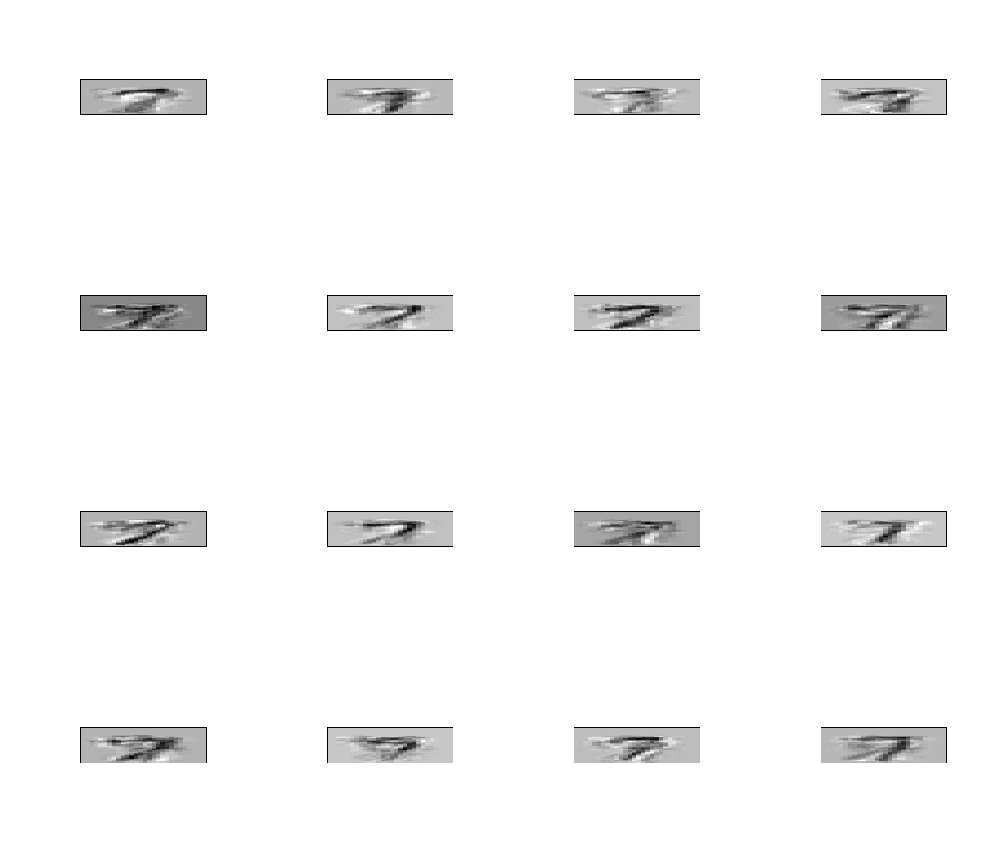
\includegraphics[width=0.8\textwidth]{samples-of-7.pdf}
%\caption{\label{fig:samples}16 samples for the digit ``7\rq\rq{}}
%\end{figure}
\end{enumerate}
\section{Multiple measurements}
$X \in \mathbb{R}$. $X \sim N(\mu_x,\lambda_0^{-1})$. $Y_1,\ldots,Y_n \in \mathbb{R}$, independent, same distribution $N(x,\lambda^{-1})$ given $x$. Consider observations $y_1,\ldots,y_n$ of $Y_1,\ldots,Y_n$.   
\begin{enumerate}
\item Compute $E[X|y_1,\ldots,y_n]$.

	\textbf{Solution:} The above distribution $N \left( x, \lambda^{-1} \right)$ applies to the random variable $Y|X=x$. That is, the variable $Y$ is the superposition of two random variables,
	\begin{equation}
		Y_i = X + \epsilon, \quad \epsilon \sim N(0, \lambda^{-1}).
	\end{equation}
	In this case, it is assumed that $\epsilon$ is independent of $X$. Hence, the following covariances follow,
	\begin{equation}
		\begin{cases}
			\operatorname{cov} (X, X) = \lambda_0^{-1}\\
			\operatorname{cov} (X, Y_i) = \lambda_0^{-1} \\
			\operatorname{cov} (Y_i, Y_j) = \lambda_0^{-1} + \lambda^{-1} \delta_{ij} \\
		\end{cases}
	\end{equation}
	The random variables $Y_1,...,Y_n$ can be augmented into a random vector $Y$, distributed as
	\begin{equation}
		Y \sim N \left( \mu_x \mathbbm 1_n, \Sigma  \right), \quad \left[ \Sigma \right]_{ij} = \begin{cases}
			\lambda_0^{-1} + \lambda^{-1}, \quad i = j \\
			\lambda_0^{-1}, \quad i \ne j \\
		\end{cases}.
	\end{equation}
Note the construction of the covariance matrix takes advantage of the independent nature of the variables. Next, it is possible to construct another vector distributed MVN,
\begin{equation} \label{eq:mvnxy}
	\begin{pmatrix}
		X \\ 
		Y \\
	\end{pmatrix} \sim
	N\left( 
		\begin{pmatrix}
			\mu_x \\ 
			\cmidrule(lr){1-1}
			\mu_x \mathbbm 1_n 
		\end{pmatrix},
		\begin{pmatrix} [c | c]
			\lambda_0^{-1} &  \lambda_0^{-1} \mathbbm 1_n^T \\
			\cmidrule(lr){1-2}
			\lambda_0^{-1} \mathbbm 1_n & \Sigma \\
		\end{pmatrix}
	\right)
\end{equation}

From this construction, it is clear that,
\begin{equation}
	\mathbb E \left[ X | y_1,...,y_n \right] = \mu_x + \lambda_0^{-1} \mathbbm 1_n^T \Sigma^{-1} \left(
		\begin{pmatrix}
			y_1 \\
			\vdots \\
			y_n \\
		\end{pmatrix}
	- \mu_x \mathbbm 1_n\right)
\end{equation}

\item Compute $Var[X|y_1,\ldots,y_n]$
	From the MVN constructed in Equation \ref{eq:mvnxy}, 
	\begin{equation}
		\operatorname{Var} \left[ X | y_1,...,y_n \right] = \lambda_0^{-1} - \lambda_0^{-1} \mathbbm 1_n^T \Sigma^{-1} \mathbbm 1_n \lambda_0^{-1}.
	\end{equation}
	
\end{enumerate}
Note: we have started this exercise in class.

\section{Brownian Bridge}
Let $W_t, t \geq 0$ be a Brownian motion process. That is 
\begin{enumerate}
\item[1)] $W_t, t\geq 0$ is a Gaussian process (GP)
\item[2)] $W_0=0$
\item[3)] $E[W_t]=0, t \geq 0$
\item[4)] $Cov[X_s,X_t]=\min(s,t), s \geq 0, t \geq 0$
\end{enumerate}
Consider the process $B_t$, the Brownian bridge, defined over the interval $0 \leq t \leq 1$ which has the distribution of $W_t$ conditioned on the event $\{W_1=w_1\}$. $B_t$ is a Gaussian process. Compute
\begin{enumerate}
\item$ E[B_t], 0 \leq t \leq 1$
	
	\textbf{Solution: }Consider a vector $\tilde X$, containing two samples from the Brownian bridge,
	\begin{equation}
		\tilde X = \begin{pmatrix}
			X_t \\
			X_1 \\
		\end{pmatrix}
		\sim N \left(
			\begin{pmatrix}
				0 \\
				0 \\
			\end{pmatrix}
		,	
		\begin{pmatrix}
			t & t \\
			t & 1 \\
		\end{pmatrix}
	\right).
	\end{equation}
The first element is a point at some time $0 \le t \le 1$. The second element is a point at $t=1$. Now, the conditional expectation and covariance can be found,
\begin{equation}
	\mathbb E \left[ X_t | X_1 = w_1 \right] = 0 + t w_1 = t w_1. \\
\end{equation}
The condition $X_1=w_1$ is one set by the Brownian bridge formulation. 

\item $Cov[B_s,B_t], 0 \leq s,t \leq 1$

	\textbf{Solution: }A Similar method can be used to find the conditional covariance,
\begin{equation}
 \begin{aligned}
 	\tilde X' = \begin{pmatrix}
 		\tilde X \\
		X_1 \\
 	\end{pmatrix}
	&\sim
	N \left( \begin{pmatrix}
		0 \\ 
		0 \\
		0 \\
	\end{pmatrix}, 
\begin{pmatrix}
	s & s & s\\
	s & t & t \\
	s & t & 1 \\
\end{pmatrix}
\right).
 \end{aligned}	
\end{equation}
Given the notation presented in lecture, the following block matrices can be defined,
\begin{equation}
	\Sigma_{11}= \begin{pmatrix}
		 s & s \\
		 s & t \\
	\end{pmatrix},
	\Sigma_{12} = \begin{pmatrix}
		s \\
		t \\
	\end{pmatrix},
	\Sigma_{22} = \begin{pmatrix}
		1 \\
	\end{pmatrix},
\end{equation}
yielding the conditional covariance,
\begin{equation}
	\operatorname{cov} \left[ \tilde X | X_1 = w_1 \right] = \begin{pmatrix}
		s(1-s) & s(1-t) \\
		s(1-t) & t(1-t) \\
	\end{pmatrix}, 0 \le s \le t \le 1.
\end{equation}
Thus, the covariance for $0 \le t,s \le 1$ is
\begin{equation}
	\operatorname{cov} \left[ B_t, B_s \right] = \operatorname{min}(t, s) \left( 1 - \operatorname{max}(t, s) \right).
\end{equation}


\item Take the case $w_1=0$. Propose an algorithm to sample from the Brownian bridge. code it. Plot 3 samples.

\begin{algorithm}
	\caption{Brownian Bridge Sample Algorithm} 
 \hspace*{\algorithmicindent} \textbf{Input} $N$ number of samples, $w_1$ values at $B_1$ \\	
 \hspace*{\algorithmicindent} \textbf{Output} $y \in \mathbb R^n$ samples of Brownian bridge $B_t$ 
 \begin{algorithmic}[1]
	 \State $X \leftarrow \{x_i = {i}/{N}, \quad i \in \mathbb Z[0, N]\}$
	 \State $[K]_{ij} \leftarrow \operatorname{min}(x_i, x_j)(1- \operatorname{max}(x_i, x_j)), \quad x_i, x_j \in X$
	 \State $[\mu]_i \leftarrow x_i w_1$  
	 \State \textbf{Return} SampleFromMultivariateGaussianDistribution$ \left( \mu, K \right)$
 \end{algorithmic}
\end{algorithm}

	\textbf{Solution: }See Figure \ref{fig:bbridge}.

\begin{figure}
	\centering
	\includegraphics[width=0.65\linewidth]{./img/bbridge.eps}
	\caption{Brownian Bridge for $w_1=0$}%
	\label{fig:bbridge}
\end{figure}
%\begin{figure}
%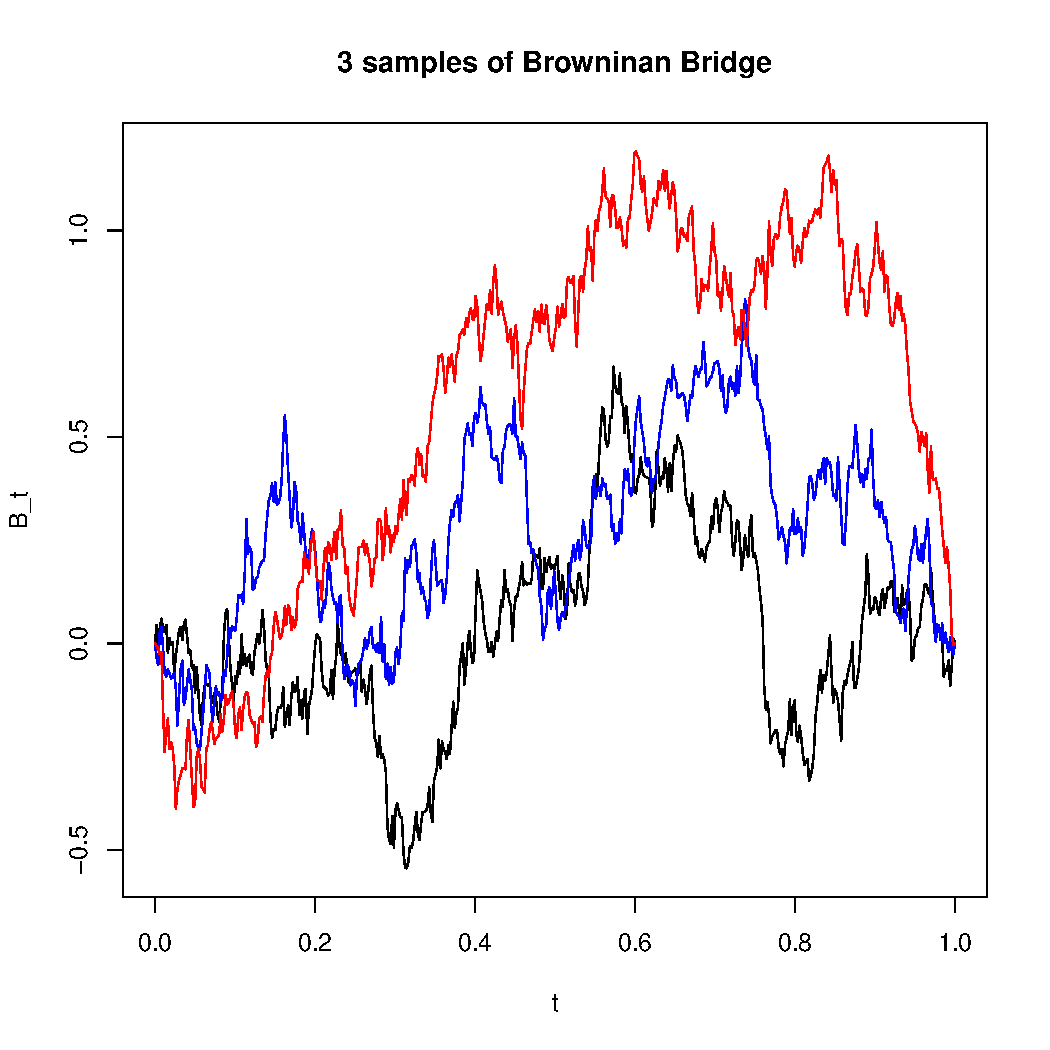
\includegraphics[width=0.5\textwidth]{BB.pdf}
%\caption{\label{fig:GB}Samples from the Gaussian Bridge}
%\end{figure}
 
\end{enumerate}
\section{Gaussian process with a linear prior}
Consider the following model. $x \in \mathbb{R}$, $k(.,.)$ is a p.d. kernel. $\beta=(\beta_1,\beta_2)^T$ is bivariate random vector.   
\begin{eqnarray}
f & \sim & GP(0,k)\\
\epsilon & \sim & GP(0,\delta) \\
\beta & \sim & N(b,\Sigma) \\
h(x) & = & (1,x)^T\\
g(x) & = & h(x)^T \beta + f(x)\\
y(x) &=& g(x) + \epsilon(x) 
\end{eqnarray}
Moreover, assume that $(f,\epsilon,\beta)$ are independent. Consider a vector of observations $y=(y_1,\ldots,y_n)$ 
\begin{enumerate}
\item Compute $E[\beta|y]$
	
	\textbf{Solution: } Construct the MVN distributed vector,
	\begin{equation}
		\begin{pmatrix}
			\beta \\
			Y \\
		\end{pmatrix}
		\sim N\left( 
\begin{pmatrix}
	b \\
	h(x)^T b \\
\end{pmatrix},
\begin{pmatrix}
	\Sigma_{11} & \Sigma_{12} \\
	\Sigma^T_{12} & \Sigma_{22} \\
\end{pmatrix}
		\right)
	\end{equation}
	Now, it is necessary to find the relevant block matrices inside the covariance matrix. Notably, consider the elements of $\Sigma_{22}$,
	\begin{equation}
	\begin{aligned}
		\left[ \Sigma_{22} \right]_{ij} &= \operatorname{cov} \left[ y(x_i), y(x_j) \right] \\
						&=  \operatorname{cov} \left[ h(x_i)^T \beta + f(x_i) + \epsilon(x_i), h(x_j)^T \beta + f(x_j) + \epsilon(x_j) \right] \\
						&= \operatorname{cov} \left[ h(x_i)^T\beta, h(x_j)^T\beta \right] + \operatorname{cov} \left[ f(x_i), f(x_j) \right] + \operatorname{cov} \left[ \epsilon(x_i), \epsilon(x_j) \right]\\
						&= \operatorname{cov} \left[ h(x_i)^T\beta, h(x_j)^T\beta \right] + k(x_i, x_j) + \delta(x_i, x_j)  
	\end{aligned}
	\end{equation}
	Manipulate the first term of the RHS,
	\begin{equation}
		\begin{aligned}
			\operatorname{cov} \left[ h(x_i)^T \beta, h(x_j)^T \beta \right] &= \operatorname{cov} \left[ \sum^{2}_{k=1} \left[ h(x_i)^T \right]_k \beta_k, \sum^{2}_{l=1} \left[ h(x_j)^T \right]_l \beta_l   \right]\\
											 &= \sum^{2}_{k=1} \sum^{2}_{l=1} \left[ h(x_i) \right]_k \left[ h(x_j) \right]_l \operatorname{cov}\left[ \beta_k, \beta_l  \right] \\
											 &= h(x_i)^T \Sigma h(x_j). \\
		\end{aligned}
	\end{equation}
	Additionally, the following matrices can be defined, and adding the terms $K, K^*$,
	\begin{equation}
		\begin{cases}
			\left[ \Sigma_{22} \right]_{ij} = h(x_i)^T \Sigma h(x_j) + k(x_i, x_j) + \delta(x_i, x_j) \\
			\Sigma_{11} = \Sigma \\
			\left[ \Sigma_{12} \right]_{:, i} = \Sigma h(x_i)  \\  
		\end{cases}
	\end{equation}
Recognizing this form, a formula can be used,	
\begin{equation}
	\mathbb E \left[ \beta | Y \right] = b + \Sigma H \left( H^T \Sigma H + K + \Delta   \right)^{-1} \left( y - H^T b \right),
\end{equation}
where 
\begin{equation}
	\begin{cases}
		\left[ K \right]_{ij} = k(x_i, x_j), \quad K \in \mathbb R^{n \times n} \\
		\left[ \Delta \right]_{ij} = \delta(x_i, x_j), \quad \Delta \in \mathbb R^{n \times n}\\
		\left[ H \right]_{:, i} = \begin{pmatrix}
			1 & x_i \\
		\end{pmatrix}^T, \quad H \in \mathbb R^{2 \times n}.
	\end{cases}
\end{equation}
Note that if $\delta$ is the Kronecker delta function, $\Delta = I$.

\item Compute $Cov[\beta|y]$

Hint: write the joint distribution of $(\beta,y)$ then use the usual formula.

\textbf{Solution: }From the above MVN vector definition,
\begin{equation}
	\operatorname{cov} \left[ \beta | Y \right] = \Sigma - \Sigma H  \left( H^T \Sigma H + K + \Delta \right)^{-1} H^T \Sigma,
\end{equation}

Consider now a new point $x^*$,
\item Compute $E[y(x^*)|y]$i
	
	\textbf{Solution: }Produce a similar construction, with
	\begin{equation}
		\begin{cases}
			\Sigma_{11} = h(x^*)^T \Sigma h(x^*) + k(x^*, x^*) + \delta(x^*, x^*) \\
			\Sigma_{12} = h(x^*)^T \Sigma H \\
			\Sigma_{22} = H^T \Sigma H + K + \Delta \\
		\end{cases}
	\end{equation}
	Accordingly, 
	\begin{equation}
		E \left[ y(x^*) | y \right] = h(x^*)^T \beta + h(x^*)^T \Sigma H \left( H^T \Sigma H + K + \Delta \right)^{-1} \left( y - H^T \beta \right).
	\end{equation}
	

\item Compute $V[y(x^*)|y]$

	\textbf{Solution: }From the previous construction,
\begin{equation}
	\begin{aligned}
		\operatorname{V} \left[ y(x^*) | y  \right] =&  h(x^*)^T \Sigma h(x^*) + k(x^*, x^*) + \delta(x^*, x^*)\\ &
		- h(x^*)^T \Sigma H  \left( H^T \Sigma H + K + \Delta \right)^{-1} H^T \Sigma h(x^*)
	\end{aligned}
\end{equation}

\end{enumerate}

\end{document}
